%%%%%%%%%%%%%%%%%%%%%%%%%%%%%%%%%%%%%%%%%
% Structured General Purpose Assignment
% LaTeX Template
%
% This template has been downloaded from:
% http://www.latextemplates.com
%
% Original author:
% Ted Pavlic (http://www.tedpavlic.com)
%
% Note:
% The \lipsum[#] commands throughout this template generate dummy text
% to fill the template out. These commands should all be removed when 
% writing assignment content.
%
%%%%%%%%%%%%%%%%%%%%%%%%%%%%%%%%%%%%%%%%%

%----------------------------------------------------------------------------------------
%	PACKAGES AND OTHER DOCUMENT CONFIGURATIONS
%----------------------------------------------------------------------------------------

\documentclass{article}

\usepackage{listings}
\usepackage{mathtools}
\usepackage{fancyhdr} % Required for custom headers
\usepackage{lastpage} % Required to determine the last page for the footer
\usepackage{extramarks} % Required for headers and footers
\usepackage{graphicx} % Required to insert images
\usepackage{lipsum} % Used for inserting dummy 'Lorem ipsum' text into the template
\usepackage{caption}
\usepackage{subcaption}
\usepackage{amsmath}

% Margins
\topmargin=-0.45in
\evensidemargin=0in
\oddsidemargin=0in
\textwidth=6.5in
\textheight=9.0in
\headsep=0.25in 

\linespread{1.1} % Line spacing

% Set up the header and footer
\pagestyle{fancy}
\lhead{\hmwkAuthorName} % Top left header
\chead{\hmwkClass} % Top center header   -->  \ (\hmwkClassInstructor\ \hmwkClassTime): \hmwkTitle
\rhead{\firstxmark} % Top right header
\lfoot{\lastxmark} % Bottom left footer
\cfoot{} % Bottom center footer
\rfoot{Page\ \thepage\ of\ \pageref{LastPage}} % Bottom right footer
\renewcommand\headrulewidth{0.4pt} % Size of the header rule
\renewcommand\footrulewidth{0.4pt} % Size of the footer rule

\setlength\parindent{0pt} % Removes all indentation from paragraphs

%----------------------------------------------------------------------------------------
%	DOCUMENT STRUCTURE COMMANDS
%	Skip this unless you know what you're doing
%----------------------------------------------------------------------------------------

% Header and footer for when a page split occurs within a problem environment
\newcommand{\enterProblemHeader}[1]{
\nobreak\extramarks{#1}{#1 continued on next page\ldots}\nobreak
\nobreak\extramarks{#1 (continued)}{#1 continued on next page\ldots}\nobreak
}

% Header and footer for when a page split occurs between problem environments
\newcommand{\exitProblemHeader}[1]{
\nobreak\extramarks{#1 (continued)}{#1 continued on next page\ldots}\nobreak
\nobreak\extramarks{#1}{}\nobreak
}

\setcounter{secnumdepth}{0} % Removes default section numbers
\newcounter{homeworkProblemCounter} % Creates a counter to keep track of the number of problems

\newcommand{\homeworkProblemName}{}
\newenvironment{homeworkProblem}[1][Problem \arabic{homeworkProblemCounter}]{ % Makes a new environment called homeworkProblem which takes 1 argument (custom name) but the default is "Problem #"
\stepcounter{homeworkProblemCounter} % Increase counter for number of problems
\renewcommand{\homeworkProblemName}{#1} % Assign \homeworkProblemName the name of the problem
\section{\homeworkProblemName} % Make a section in the document with the custom problem count
\enterProblemHeader{\homeworkProblemName} % Header and footer within the environment
}{
\exitProblemHeader{\homeworkProblemName} % Header and footer after the environment
}

\newcommand{\problemAnswer}[1]{ % Defines the problem answer command with the content as the only argument
\noindent\framebox[\columnwidth][c]{\begin{minipage}{0.98\columnwidth}#1\end{minipage}} % Makes the box around the problem answer and puts the content inside
}

\newcommand{\homeworkSectionName}{}
\newenvironment{homeworkSection}[1]{ % New environment for sections within homework problems, takes 1 argument - the name of the section
\renewcommand{\homeworkSectionName}{#1} % Assign \homeworkSectionName to the name of the section from the environment argument
\subsection{\homeworkSectionName} % Make a subsection with the custom name of the subsection
\enterProblemHeader{\homeworkProblemName\ [\homeworkSectionName]} % Header and footer within the environment
}{
\enterProblemHeader{\homeworkProblemName} % Header and footer after the environment
}
   
%----------------------------------------------------------------------------------------
%	NAME AND CLASS SECTION
%----------------------------------------------------------------------------------------

\newcommand{\hmwkTitle}{Project\ \#4} % Assignment title
\newcommand{\hmwkDueDate}{Tuesday,\ April\ 21,\ 2015} % Due date
\newcommand{\hmwkClass}{CSCI\ 8810} % Course/class
\newcommand{\hmwkClassTime}{08:00am} % Class/lecture time
\newcommand{\hmwkClassInstructor}{Prof. Arabnia} % Teacher/lecturer
\newcommand{\hmwkAuthorName}{Sina Solaimanpour} % Your name

%----------------------------------------------------------------------------------------
%	TITLE PAGE
%----------------------------------------------------------------------------------------

\title{
\vspace{2in}
\textmd{\textbf{\hmwkClass:\ \hmwkTitle}}\\
\normalsize\vspace{0.1in}\small{Due\ on\ \hmwkDueDate}\\
\vspace{0.1in}\large{\textit{\hmwkClassInstructor\ \hmwkClassTime}}
\vspace{3in}
}

\author{\textbf{\hmwkAuthorName}}
\date{} % Insert date here if you want it to appear below your name

%----------------------------------------------------------------------------------------

\begin{document}

\maketitle

%----------------------------------------------------------------------------------------
%	TABLE OF CONTENTS
%----------------------------------------------------------------------------------------

%\setcounter{tocdepth}{1} % Uncomment this line if you don't want subsections listed in the ToC

\newpage
\tableofcontents
\newpage

%----------------------------------------------------------------------------------------
%	Introduction
%----------------------------------------------------------------------------------------

% To have just one problem per page, simply put a \clearpage after each problem

\begin{homeworkProblem}[\Roman{homeworkProblemCounter}. Introduction]
In this iteration of the ColonD (:D) Image Processor project, I am going to implement a Steganography feature to  hide a subject image in a cover image. The following sections will be talking about this feature and the experiments I did on the Steganographer I implemented. An screenshot of the program can be seen in \textbf{Figure \ref{fig:screenshot}}.

\begin{figure}[h!]
  \centering
	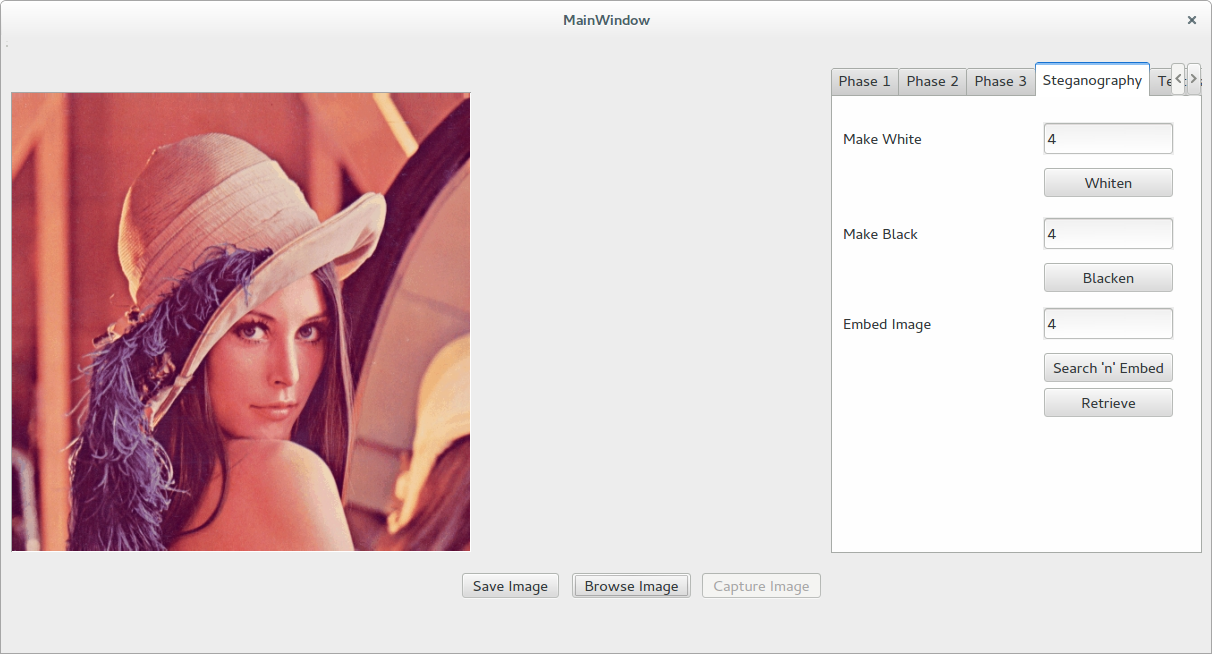
\includegraphics[width=0.7\textwidth]{pic/screenshot}
  \caption{Screenshot of the program with the new features implemented in this iteration of the project.}
  \label{fig:screenshot}
\end{figure}

\end{homeworkProblem}

%----------------------------------------------------------------------------------------
%	Whiten and Blacken
%----------------------------------------------------------------------------------------

% To have just one problem per page, simply put a \clearpage after each problem

\begin{homeworkProblem}[\Roman{homeworkProblemCounter}. Make Lower N bits White or Black]

As an extra feature, to illustrate how the number of bits chosen to hide the subject image impacts the quality of the cover image I implemented this. This feature will whiten out or blacken out the lower N bits of the image in all three RGB channels. In \textbf{Figure \ref{fig:white}} you can see results for different N values when whitening the bits and in \textbf{Figure \ref{fig:black}} you can see the results for the exact N values but with blacken bits.

\begin{figure}[h!]
  \centering
	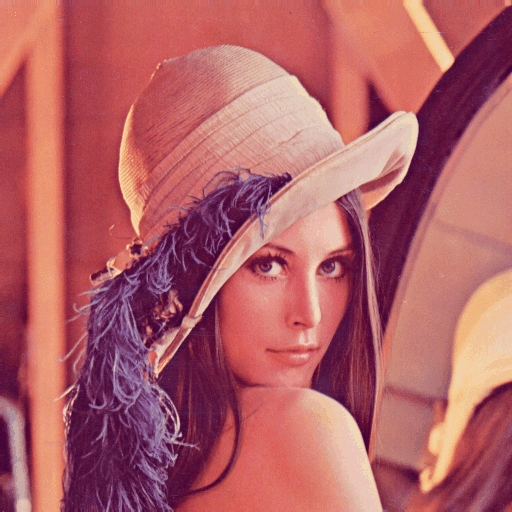
\includegraphics[width=0.3\textwidth]{pic/whiteN1}
	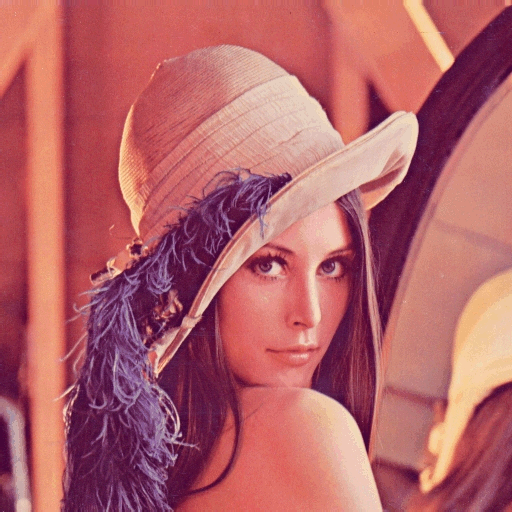
\includegraphics[width=0.3\textwidth]{pic/whiteN2}
	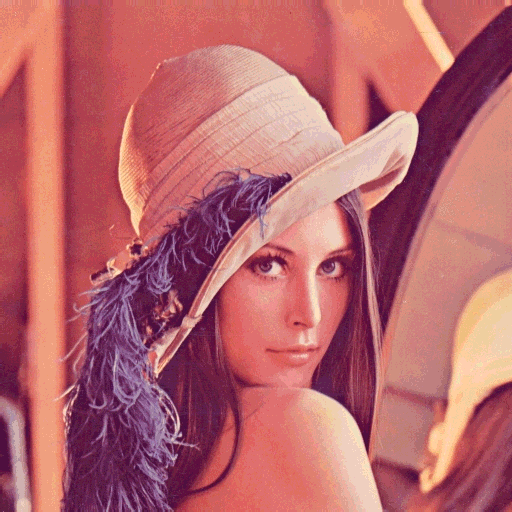
\includegraphics[width=0.3\textwidth]{pic/whiteN3}
	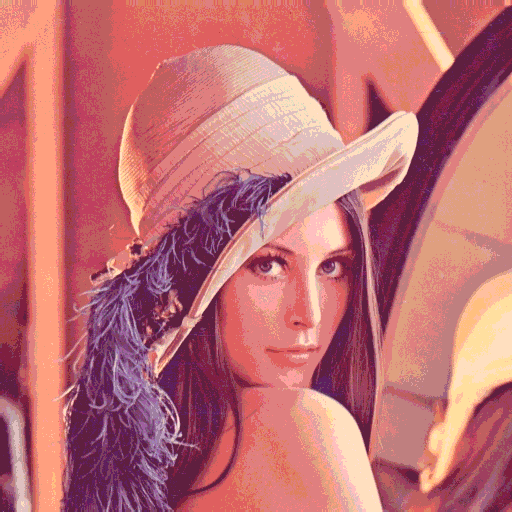
\includegraphics[width=0.3\textwidth]{pic/whiteN4}
	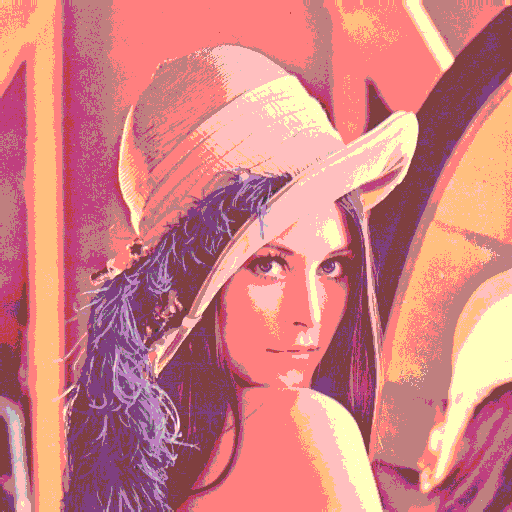
\includegraphics[width=0.3\textwidth]{pic/whiteN5}
	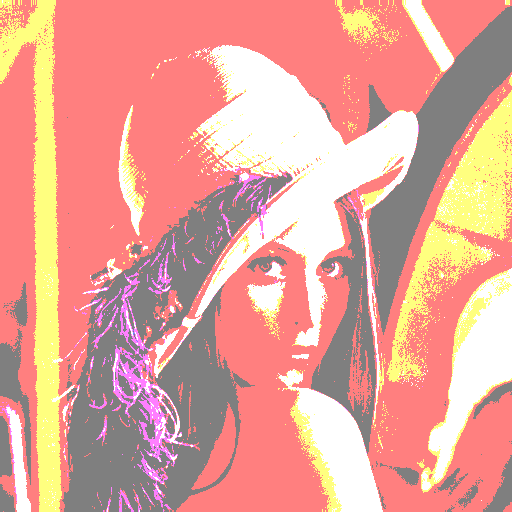
\includegraphics[width=0.3\textwidth]{pic/whiteN6}
  \caption{Results of applying different N values to the whiten feature. As you can see the effects of the whitening starts to appear from the 4th image and the 7th image is completely whitened which is removed in this report to save some space.}
  \label{fig:white}
\end{figure}

\begin{figure}[h!]
  \centering
	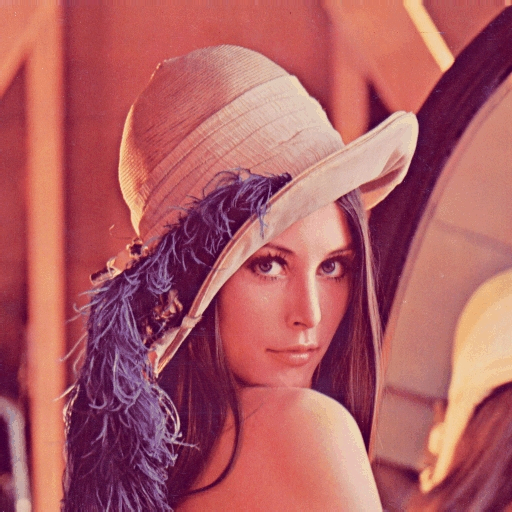
\includegraphics[width=0.3\textwidth]{pic/blackN1}
	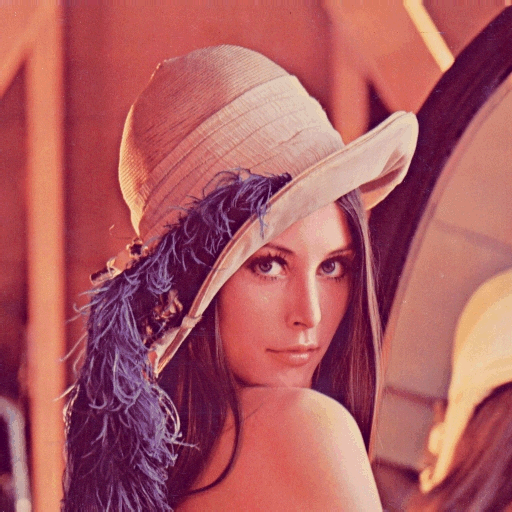
\includegraphics[width=0.3\textwidth]{pic/blackN2}
	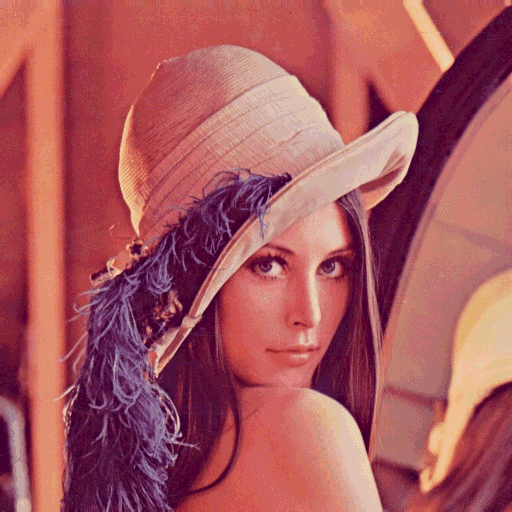
\includegraphics[width=0.3\textwidth]{pic/blackN3}
	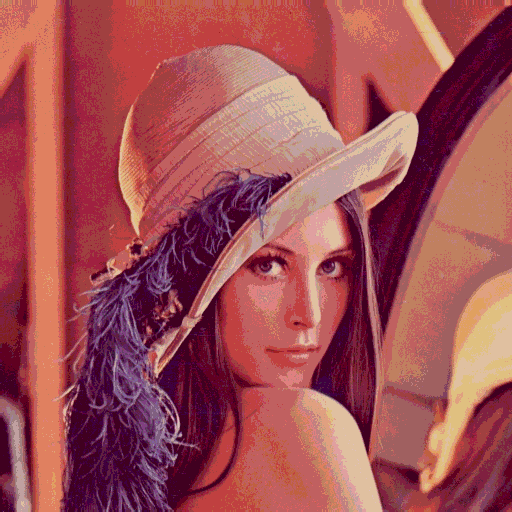
\includegraphics[width=0.3\textwidth]{pic/blackN4}
	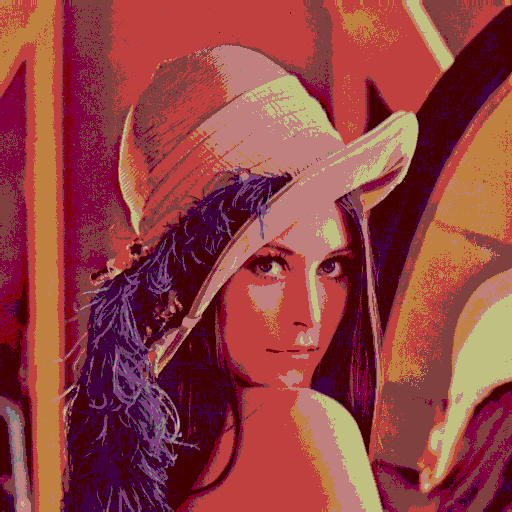
\includegraphics[width=0.3\textwidth]{pic/blackN5}
	
\includegraphics[width=0.3\textwidth]{pic/blackN6}
	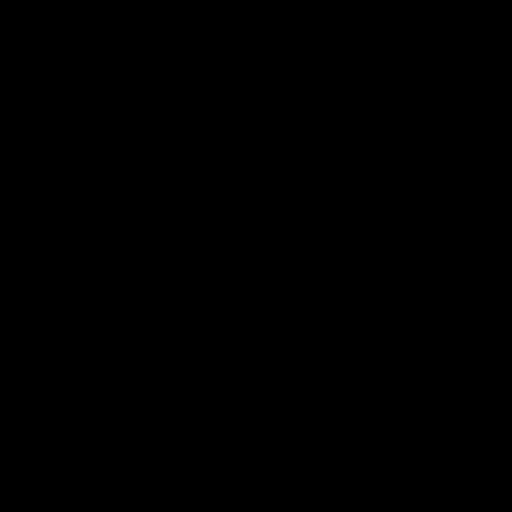
\includegraphics[width=0.3\textwidth]{pic/blackN7}
  \caption{Results of applying different N values to the blacken feature. As you can see the effects of the blackening starts to appear from the 4th image and the 7th image is completely blackened.}
  \label{fig:black}
\end{figure}

This shows that in this particular image we can hide 512x513x3 bits of information without any change in the appearance of the cover image. This number is calculated by multiplying the width by the height of the image and the number of bits whitened or blackened without seeing any effects in the image which was 3 bits. This value can be very big for large pictures taken even by old phone cameras which are typically 5 mega pixels. The amount of data that can be hidden in a 5 mega pixel image is about \textbf{15 mega bits = 1875 Kilobytes} when using only 3 lower bits of the pixel values. This amount can hide 1875 characters in it, which is more than enough for transmitting a secret message.

\end{homeworkProblem}

%----------------------------------------------------------------------------------------
%	Steganography
%----------------------------------------------------------------------------------------

% To have just one problem per page, simply put a \clearpage after each problem

\begin{homeworkProblem}[\Roman{homeworkProblemCounter}. Steganography]

After implementing the above features and doing some experiments with those two features, I decided to implement the main feature which is the steganographer. To do the steganography, I assume that the image sizes are equal and I consider both of them as color images. The user has an option to choose how many bits he/she wants to use to hide the subject image. After deciding about the N value, I take the N higher bits of the subject image and replace the N lower bits of the cover image. In \textbf{Figure \ref{fig:steg1}} you can see the resulting image from hiding the bike image in the lena's image using 3 bits. You can also see the original images and the recovered image after the process. The same images just with the N values equal to 4 is shown in \textbf{Figure \ref{fig:steg2}}. As you can see, there exists a shadow of the bike image in the resulting image with N = 4. The experiment is repeated with the same images but with N = 5 in \textbf{Figure \ref{fig:steg3}}. The resulting cover image is obviously showing that there is something going around in it but the recovered image is as if no data is damaged in it.

\begin{figure}[h!]
  \centering
	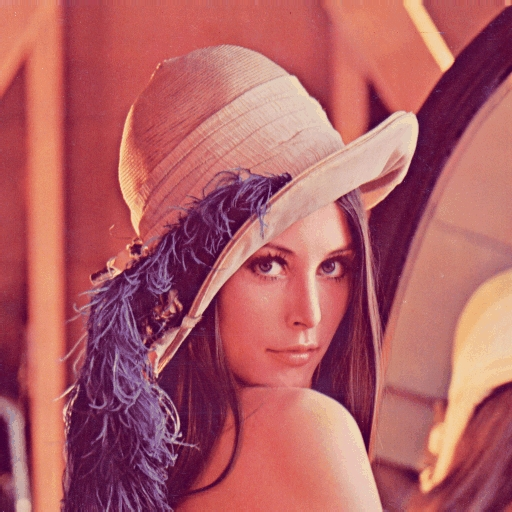
\includegraphics[width=0.23\textwidth]{pic/steg1_len}
	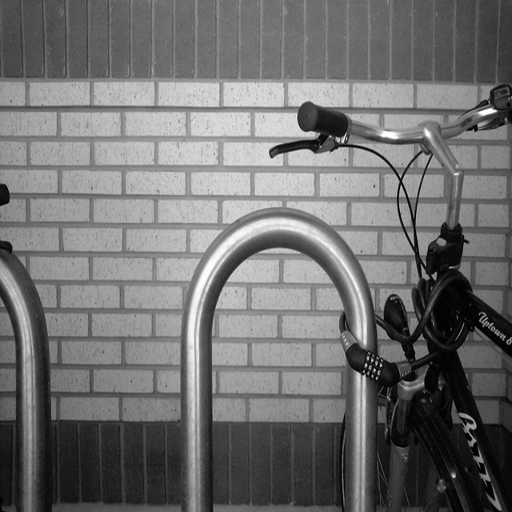
\includegraphics[width=0.23\textwidth]{pic/steg1_bike}
	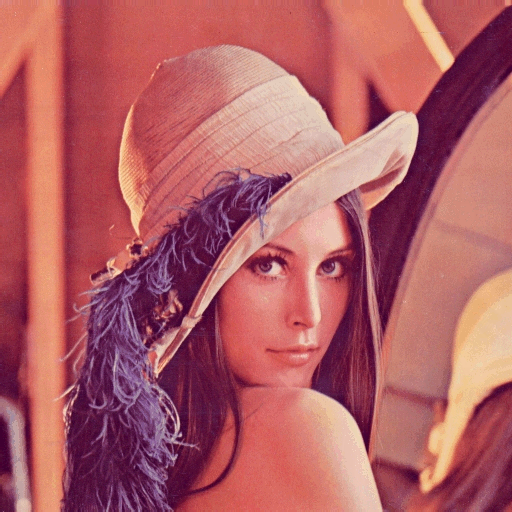
\includegraphics[width=0.23\textwidth]{pic/steg1_res}
	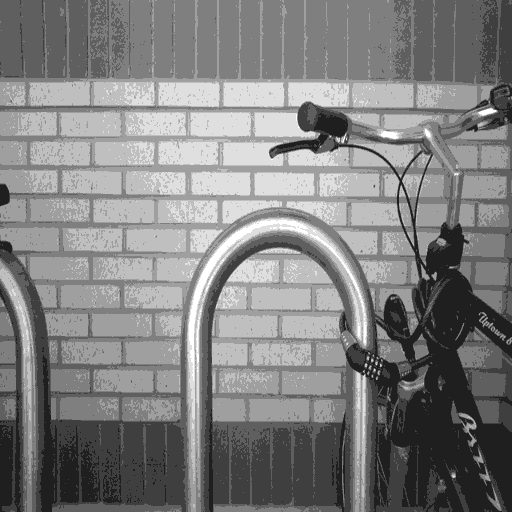
\includegraphics[width=0.23\textwidth]{pic/steg1_retr}
  \caption{The images in this figure are respectively, the original lena's picture, original bike picture, the resulting cover image with the bike image hidden in it with N = 3 and the last image is the retrieved image.}
  \label{fig:steg1}
\end{figure}

\begin{figure}[h!]
  \centering
	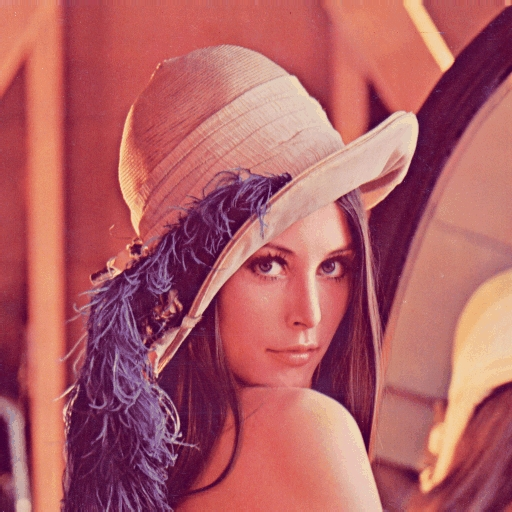
\includegraphics[width=0.23\textwidth]{pic/steg1_len}
	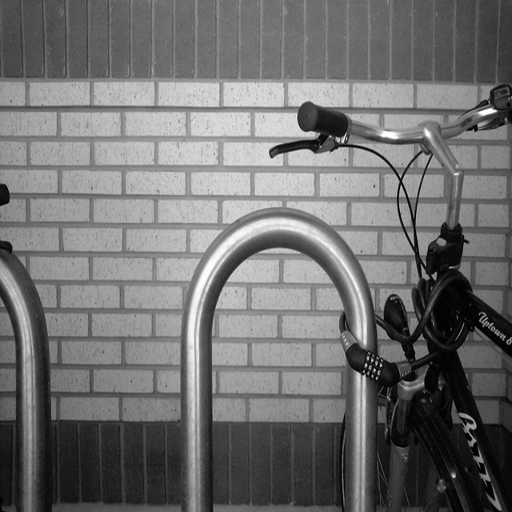
\includegraphics[width=0.23\textwidth]{pic/steg1_bike}
	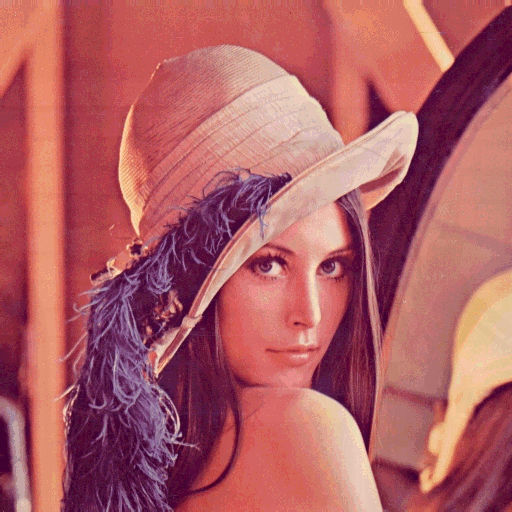
\includegraphics[width=0.23\textwidth]{pic/steg2_res}
	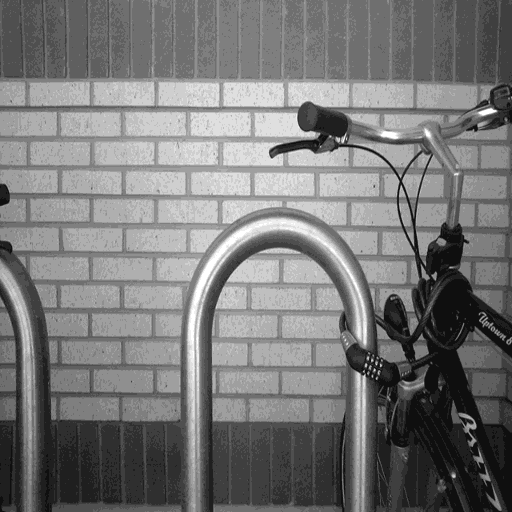
\includegraphics[width=0.23\textwidth]{pic/steg2_retr}
  \caption{The images in this figure are respectively, the original lena's picture, original bike picture, the resulting cover image with the bike image hidden in it with N = 4 and the last image is the retrieved image.}
  \label{fig:steg2}
\end{figure}

\begin{figure}[h!]
  \centering
	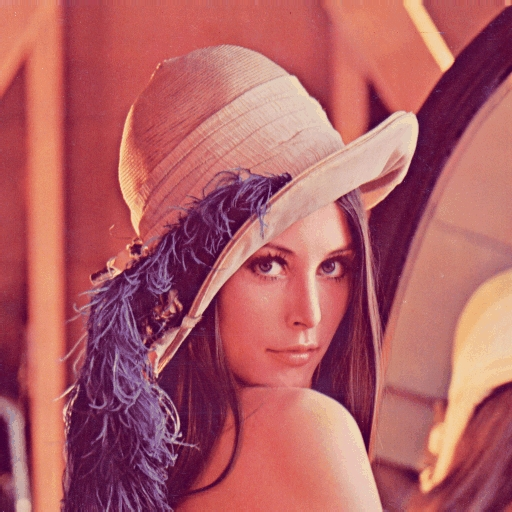
\includegraphics[width=0.23\textwidth]{pic/steg1_len}
	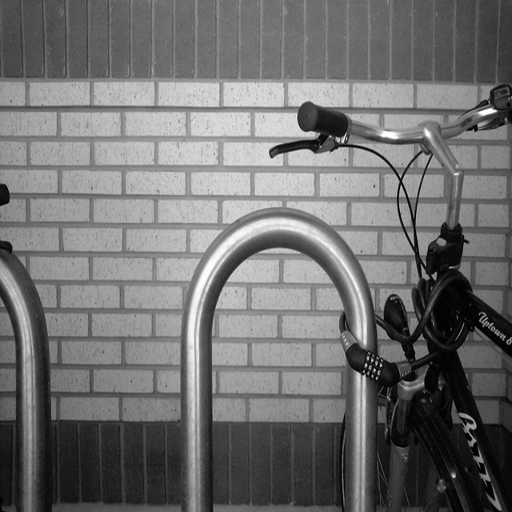
\includegraphics[width=0.23\textwidth]{pic/steg1_bike}
	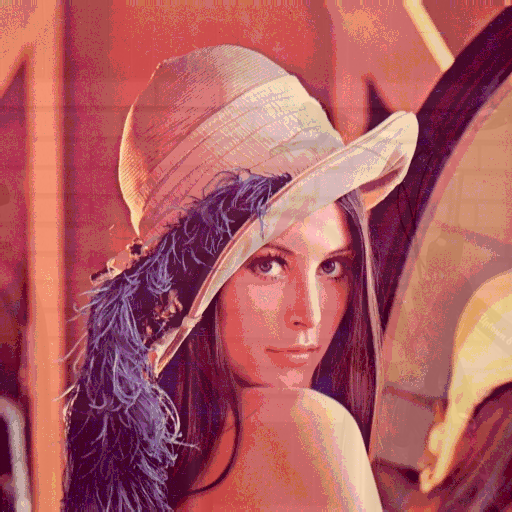
\includegraphics[width=0.23\textwidth]{pic/steg3_res}
	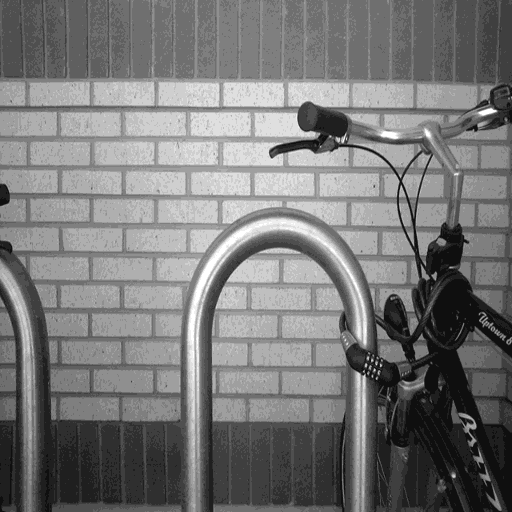
\includegraphics[width=0.23\textwidth]{pic/steg3_retr}
  \caption{The images in this figure are respectively, the original lena's picture, original bike picture, the resulting cover image with the bike image hidden in it with N = 5 and the last image is the retrieved image.}
  \label{fig:steg3}
\end{figure}

The above experiments show that N = 3 is an optimal value for N to be used with the lena's picture as the cover image. At this point, I wanted to try different images to see if this optimal value differs for different images or not. I started with an image with high change frequencies.

\end{homeworkProblem}

%----------------------------------------------------------------------------------------
%	Experiments
%----------------------------------------------------------------------------------------

% To have just one problem per page, simply put a \clearpage after each problem

\begin{homeworkProblem}[\Roman{homeworkProblemCounter}. Experiments]
I suspected that the N = 3 is a very small number and there might be some images that can be used as cover image and can handle more than N = 3 bits to be removed from their pixel values. I tried to find a picture with high frequency in changes or better say with a chaotic pattern. The \textbf{Figure \ref{fig:exp1}} shows this image which is a picture of some birds (probably sea gulls) flying with the blue sky in the background. I also created a test image to use as the subject image which simply has three sentences in it saying "MSG TO TRANSFER!!!". I used N = 5 to hide this image in the cover image and the resulting image and the recovered image is shown in the \textbf{Figure \ref{fig:exp1}}. As you can see, there's not much difference between the original image and the resulting cover image as the change frequency is very high in the original image and the subject image is a simple one. Even though I used 5 lower bits of the original image, still, there is very little effects of the steganography visible in the resulting image. This experiment shows that, the more complex and sophisticated pattern the cover image contains, the more number of bits one might be able to use to hide other information. Also, if the data which needs to be hidden in the cover image is a simple image might have some impacts on the N value.

\begin{figure}[h!]
  \centering
	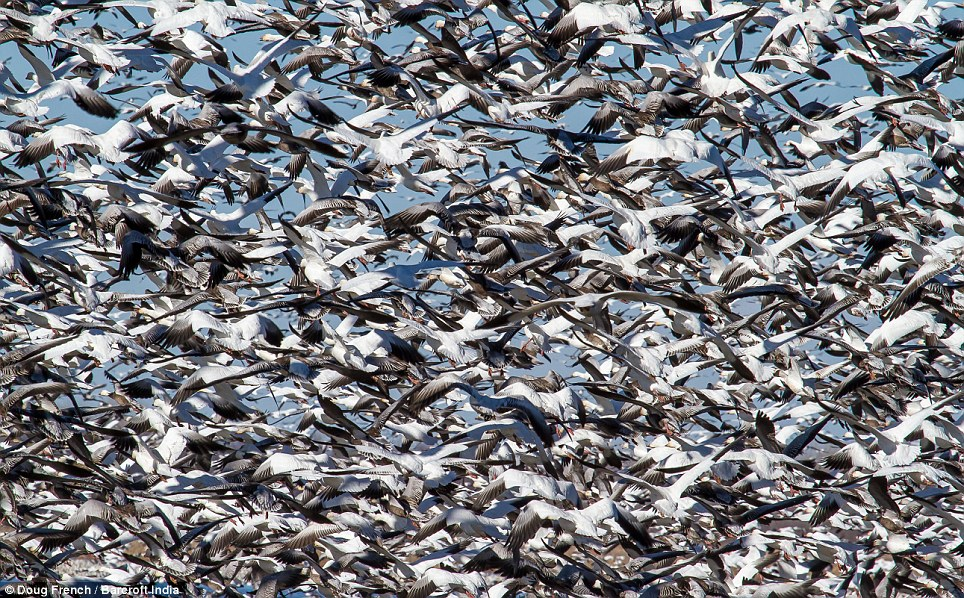
\includegraphics[width=0.3\textwidth]{pic/exp1_orig}
	
\includegraphics[width=0.3\textwidth]{pic/exp1_sub}
	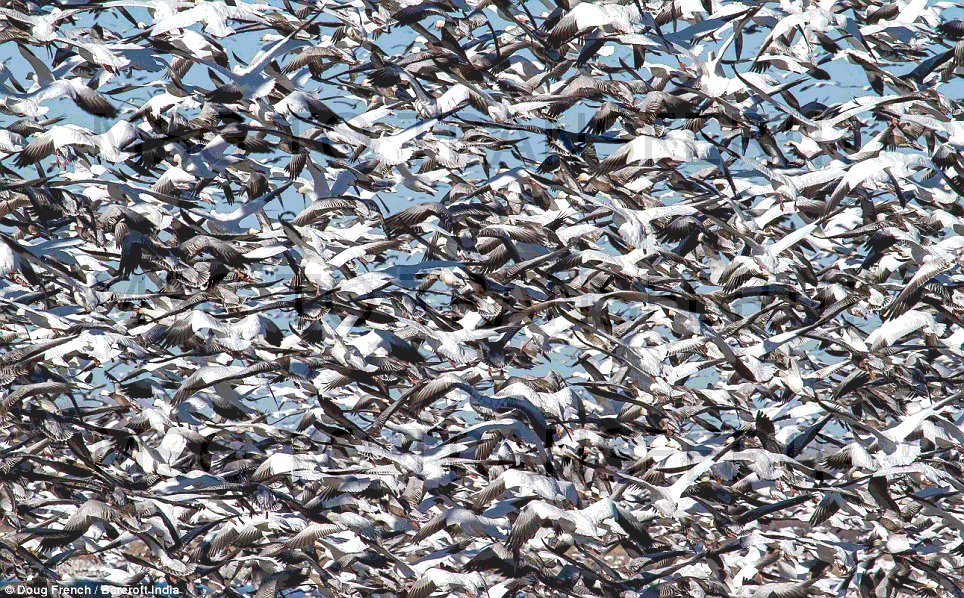
\includegraphics[width=0.3\textwidth]{pic/exp1_res}
	
\includegraphics[width=0.3\textwidth]{pic/exp1_retr}
  \caption{The experiment showing that we can use higher values for N and without showing any visible effect in the resulting image. From left to right: The original cover image, The subject image to be hidden, The resulting cover image, The retrieved image.}
  \label{fig:exp1}
\end{figure}

\end{homeworkProblem}

%----------------------------------------------------------------------------------------
%	Experiments
%----------------------------------------------------------------------------------------

% To have just one problem per page, simply put a \clearpage after each problem

\begin{homeworkProblem}[\Roman{homeworkProblemCounter}. Suggestions]
As for suggestions to make it more difficult for the cracker to recover the hidden image, I can say that we can use a pattern to put the subject data inside the original image instead of just storing the data in the same order as it was in the original image. This can scramble the recovered data and make a little more difficult for the cracker to figure out the pattern. Also, we can use variable bits to store the data such that, by having a pattern, we can change the number of bits that we use in the pixel value in the cover image to hide the subject data. This might also help in hiding the data more effectively. 

Breaking up the data into multiple images, encrypting the data and then storing them and many other ways of data hiding techniques can be used in this application.

\end{homeworkProblem}


\end{document}
